\documentclass[xcolor=dvipsnames]{beamer}
\usetheme{nelle}
\usepackage{natbib}                 % Fancy bibliography.
\usepackage{url}                    % Allow printing of URLs.
\usepackage{outlines}
\usepackage{enumitem}
\usepackage{multicol}
\usepackage{dsfont}
\usepackage{amsmath}
\usepackage{epstopdf}
\usepackage{color}
\usepackage{booktabs}
\setbeamerfont{caption}{size=\scriptsize}
\setbeamertemplate{navigation symbols}{}
\setbeamertemplate{footline}[frame number]{}

\def\newblock{\hskip .11em plus .33em minus .07em}

\title{\textbf{Analysing time-course gene expression data to understand
drought tolerance in plants}}

\author[Varoquaux Nelle]{Nelle Varoquaux}


\date{November, 5th}
\institute{CNRS, TIMC, Grenoble}
\begin{document}
\begin{frame}[t, noframenumbering]
  \maketitle

\end{frame}

\setcounter{framenumber}{0}

\section{Transcriptomics in the EPICON project}

\begin{frame}
\frametitle{Drought, one of the most severe environmental threat}
\begin{center}
\vspace{-2.3em}
\hspace*{-3em}
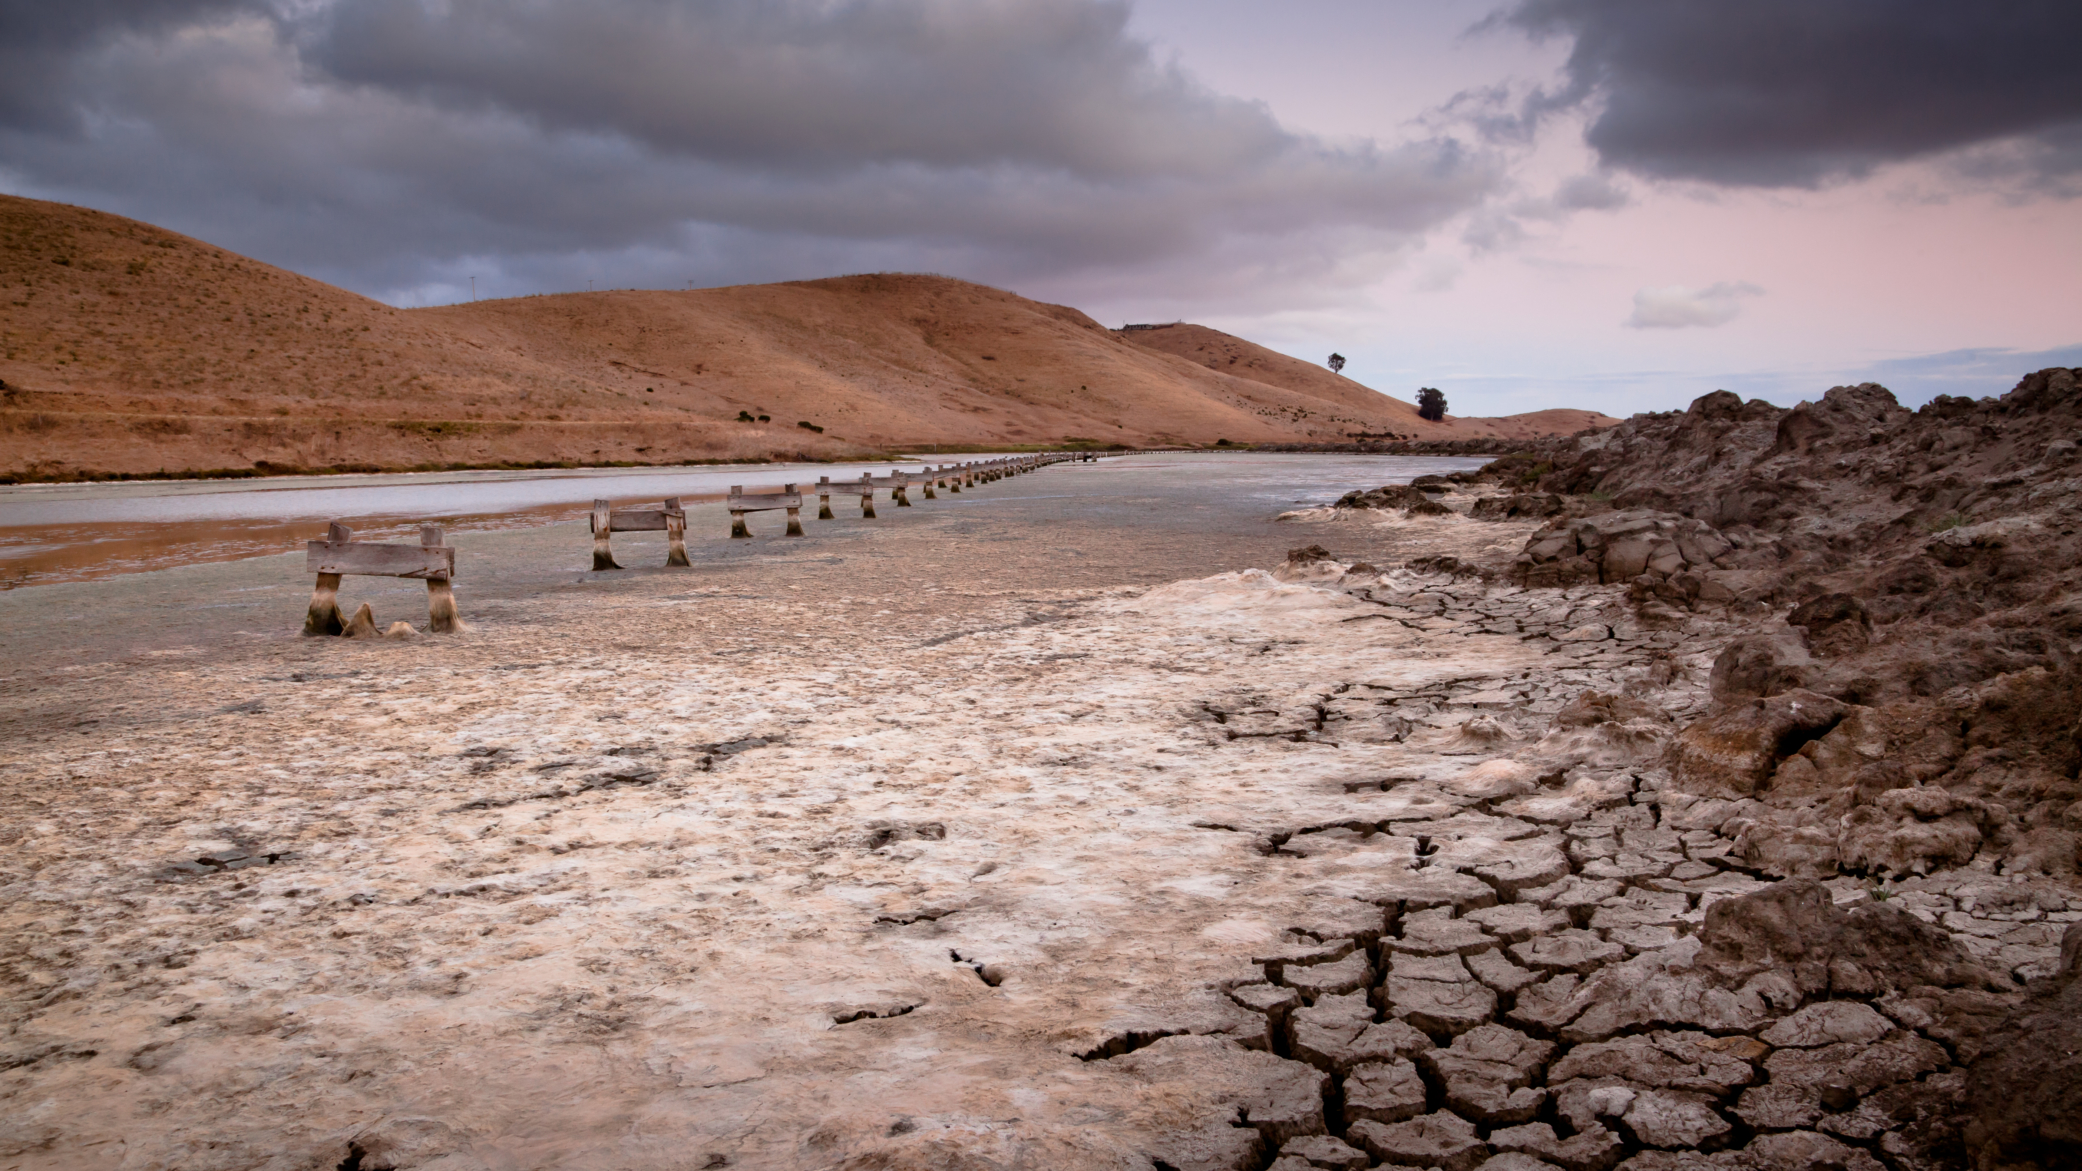
\includegraphics[width=1.5\linewidth]{images/drought.jpg}
\end{center}
\end{frame}

\begin{frame}
\frametitle{Water challenges in California}
\begin{columns}
\begin{column}{0.5\linewidth}
\begin{flushright}
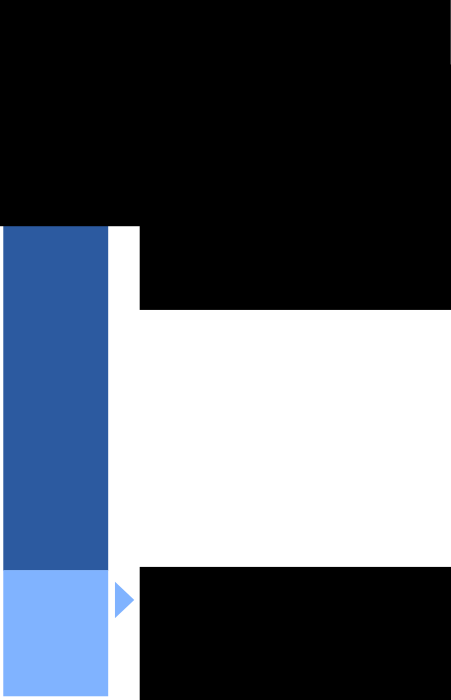
\includegraphics[width=0.7\linewidth]{images/water_california.pdf}
\end{flushright}
\end{column}
\begin{column}{0.5\linewidth}
By 2030, California will have an unmet water demand of 1.5 trillions gallons an
average year, and more in a dry year.
\end{column}
\end{columns}
\begin{flushright}
\tiny
Source: California Water Challenge
\end{flushright}
\end{frame}

\begin{frame}
\frametitle{How to tackle the issue of drought in California?}
\begin{center}
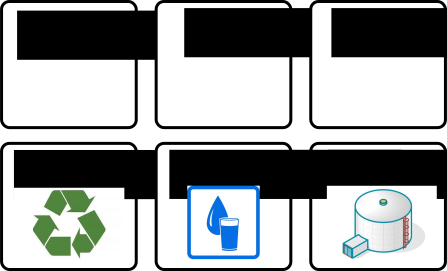
\includegraphics[width=0.8\linewidth]{images/water_solution.pdf}
\end{center}
\end{frame}


\begin{frame}
\frametitle{}
\vspace{7em}
{\Large Better understanding the dynamical response of plants under drought
stress.}

\vspace{3em}
\begin{center}
\hspace*{-1.5em}

\includegraphics[width=1.1\linewidth]{images/plant_drought_stress.jpg}
\end{center}
\end{frame}


\begin{frame}
\frametitle{Exploring \textit{S. bicolor}'s incredible drought tolerance
property}
  

\textbf{\color{Blue} Goal} \quad generate a model linking physiology and
genetics of
  \textit{S. bicolor} with its \textbf{epigenetic regulatory machinery}, the
  dynamics of its \textbf{microbial community} and the composite
\textbf{genetic pathways involved in drought response}.
  
  \vspace{1em}
  \textbf{\color{Blue} Idea} \quad Field experiment under different drought
conditions to
  collect data to generate a model for drought acclimatation.

\begin{center}
\hspace*{-1.5em}
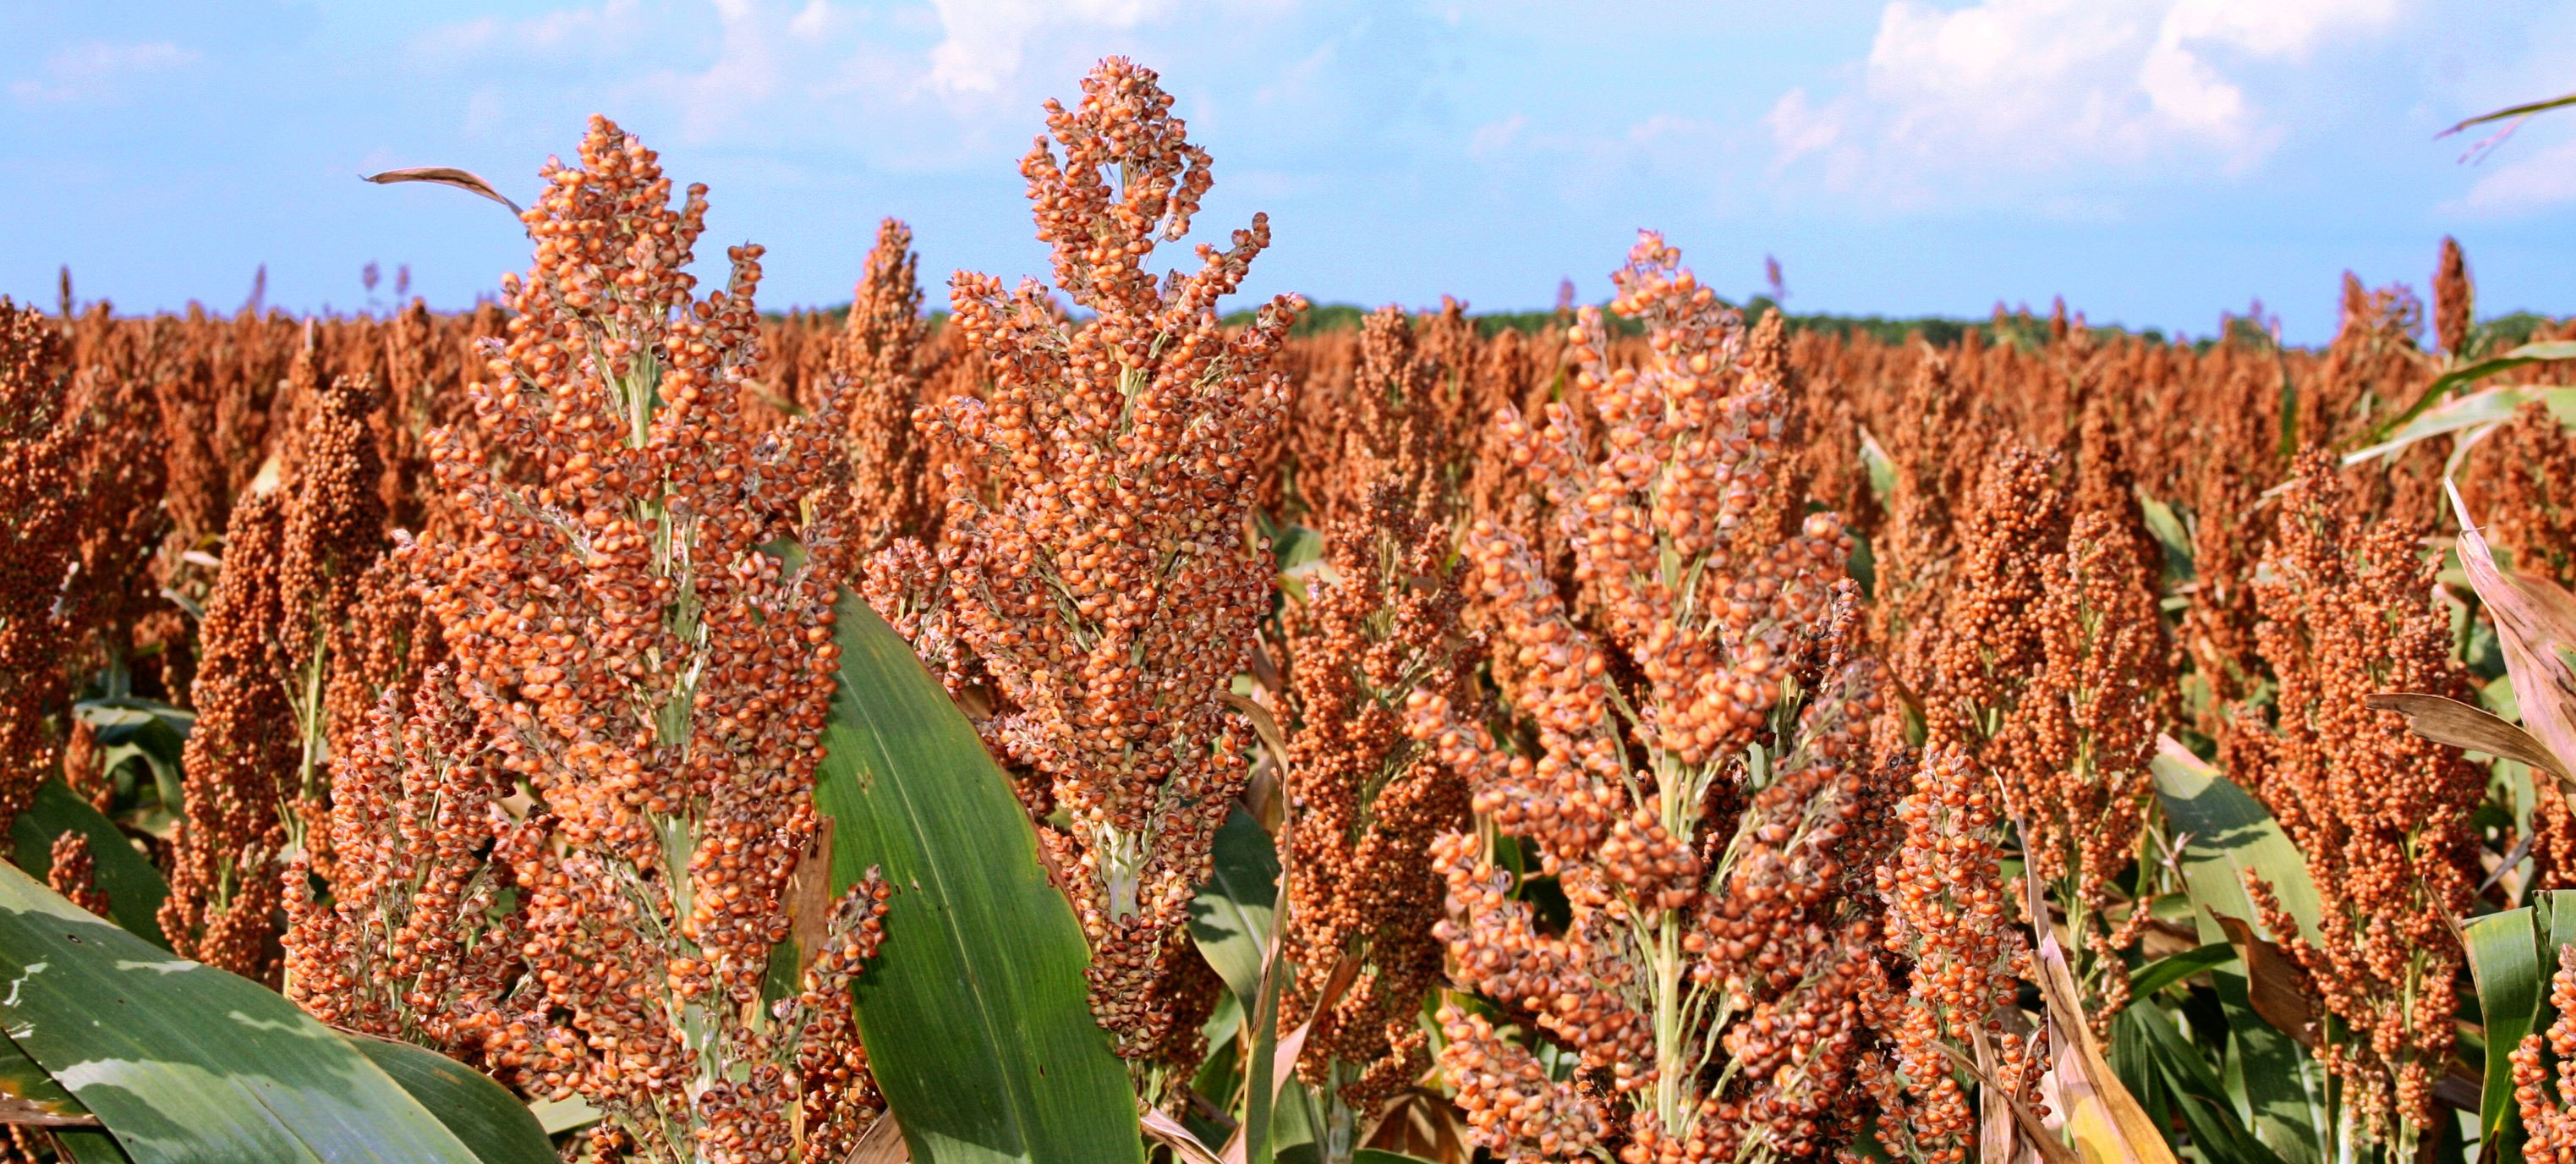
\includegraphics[width=1.1\linewidth]{images/sorghum.jpg}
\end{center}

\end{frame}
  
\begin{frame}
\frametitle{EPICON:\ the experiment}

\textbf{\color{Blue} In brief}\\
\begin{figure}
\centering
\begin{minipage}{0.15\textwidth}
\begin{flushright}
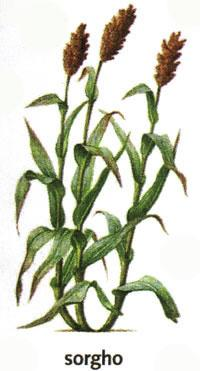
\includegraphics[width=0.8\linewidth]{images/sorghum.png}
\end{flushright}
\end{minipage}
\begin{minipage}{0.5\textwidth}
\begin{center}

\includegraphics[width=0.8\linewidth]{images/drought.png}
\end{center}
\caption{\bf Different drought conditions}
\end{minipage}
\begin{minipage}{0.3\textwidth}

\includegraphics[width=0.8\linewidth]{images/epigenetics.png}\\
\end{minipage}
\end{figure}

\textbf{\color{Blue} The sampling plan}\\
\begin{figure}
\vspace{-3em}
\includegraphics[width=0.7\linewidth]{images/sampling_plan.pdf}
\caption{mRNASeq, Chip-seq, small RNA-seq, DNA methylation, Proteomics,
Metabolomics, Microbiome, most on leaf and root, every week for 3 months}
\end{figure}
\end{frame}  



\begin{frame}
\frametitle{The transcriptomic data}
\begin{itemize}[label={$\bullet$}]
\item Gene expression data of nearly 400 samples (RNA-seq)
\begin{itemize}[label={$\bullet$}]
\item Leaf \& Root samples
\item Three treatments: pre-flowering drought, post-flowering drought, and
well watered
\item Two genotypes: RTx430 (pre-flowering drought tolerant) \& BTx642
(stay-green and post-flowering drought tolerant)
\item Between 1 \& 3 replicates per condition
\item Sampled weekly between week 2 \& 17 
\end{itemize}
\item 30,000 genes in $S. bicolor$
\end{itemize}
\end{frame}

\begin{frame}
\frametitle{The data analysis pipeline}
\begin{center}
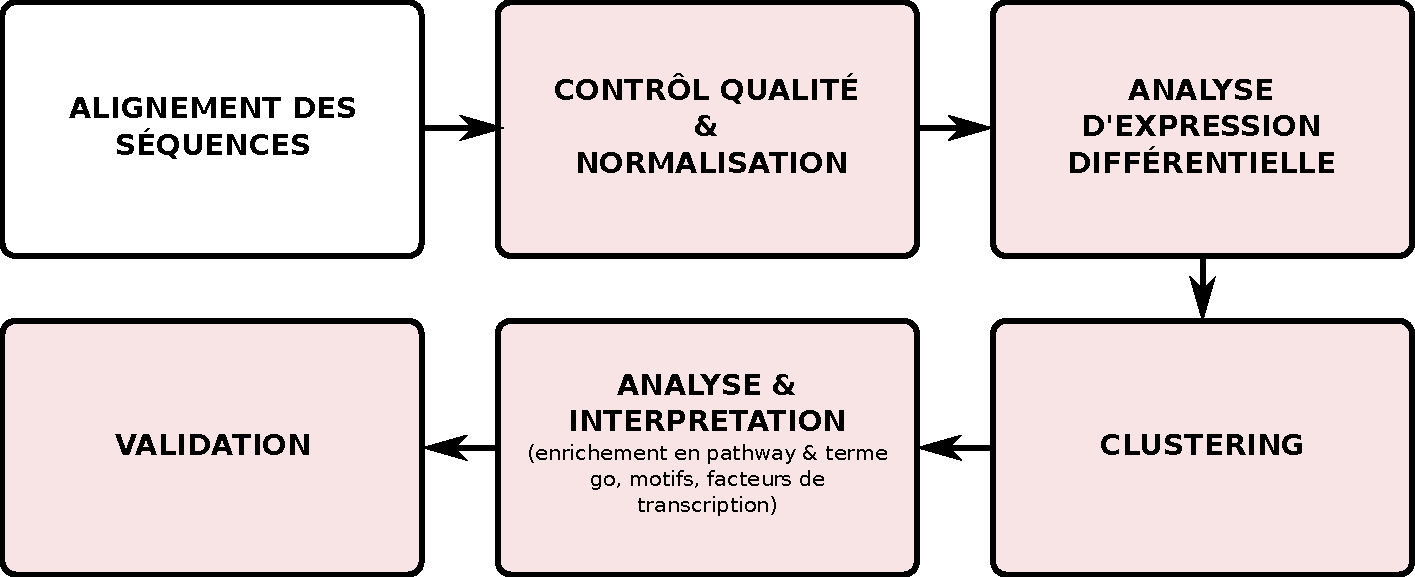
\includegraphics[width=0.9\linewidth]{images/data_analysis_pipeline.pdf}
\end{center}
\end{frame}

\begin{frame}
\frametitle{Detecting genes differentially expressed in time-course
experiments}

\textbf{\color{Blue} Goal} \quad Find which genes are implicated in \textit{S.
bicolor}'s resistance to drought. Precisely,
\begin{itemize}[label={$\bullet$}]
\item For both genotype and both type of drought condition, find which genes
are implicated in drought resistance.
\item Find which gene behave differently between both genotype.
\end{itemize}
\vspace{1em}

\textbf{\color{Blue} Idea} \quad leverage the time-course aspect of the data and the
litterature on functional analysis.
\end{frame}

\begin{frame}
\frametitle{Differential expression analysis in a classic gene expression experiment}
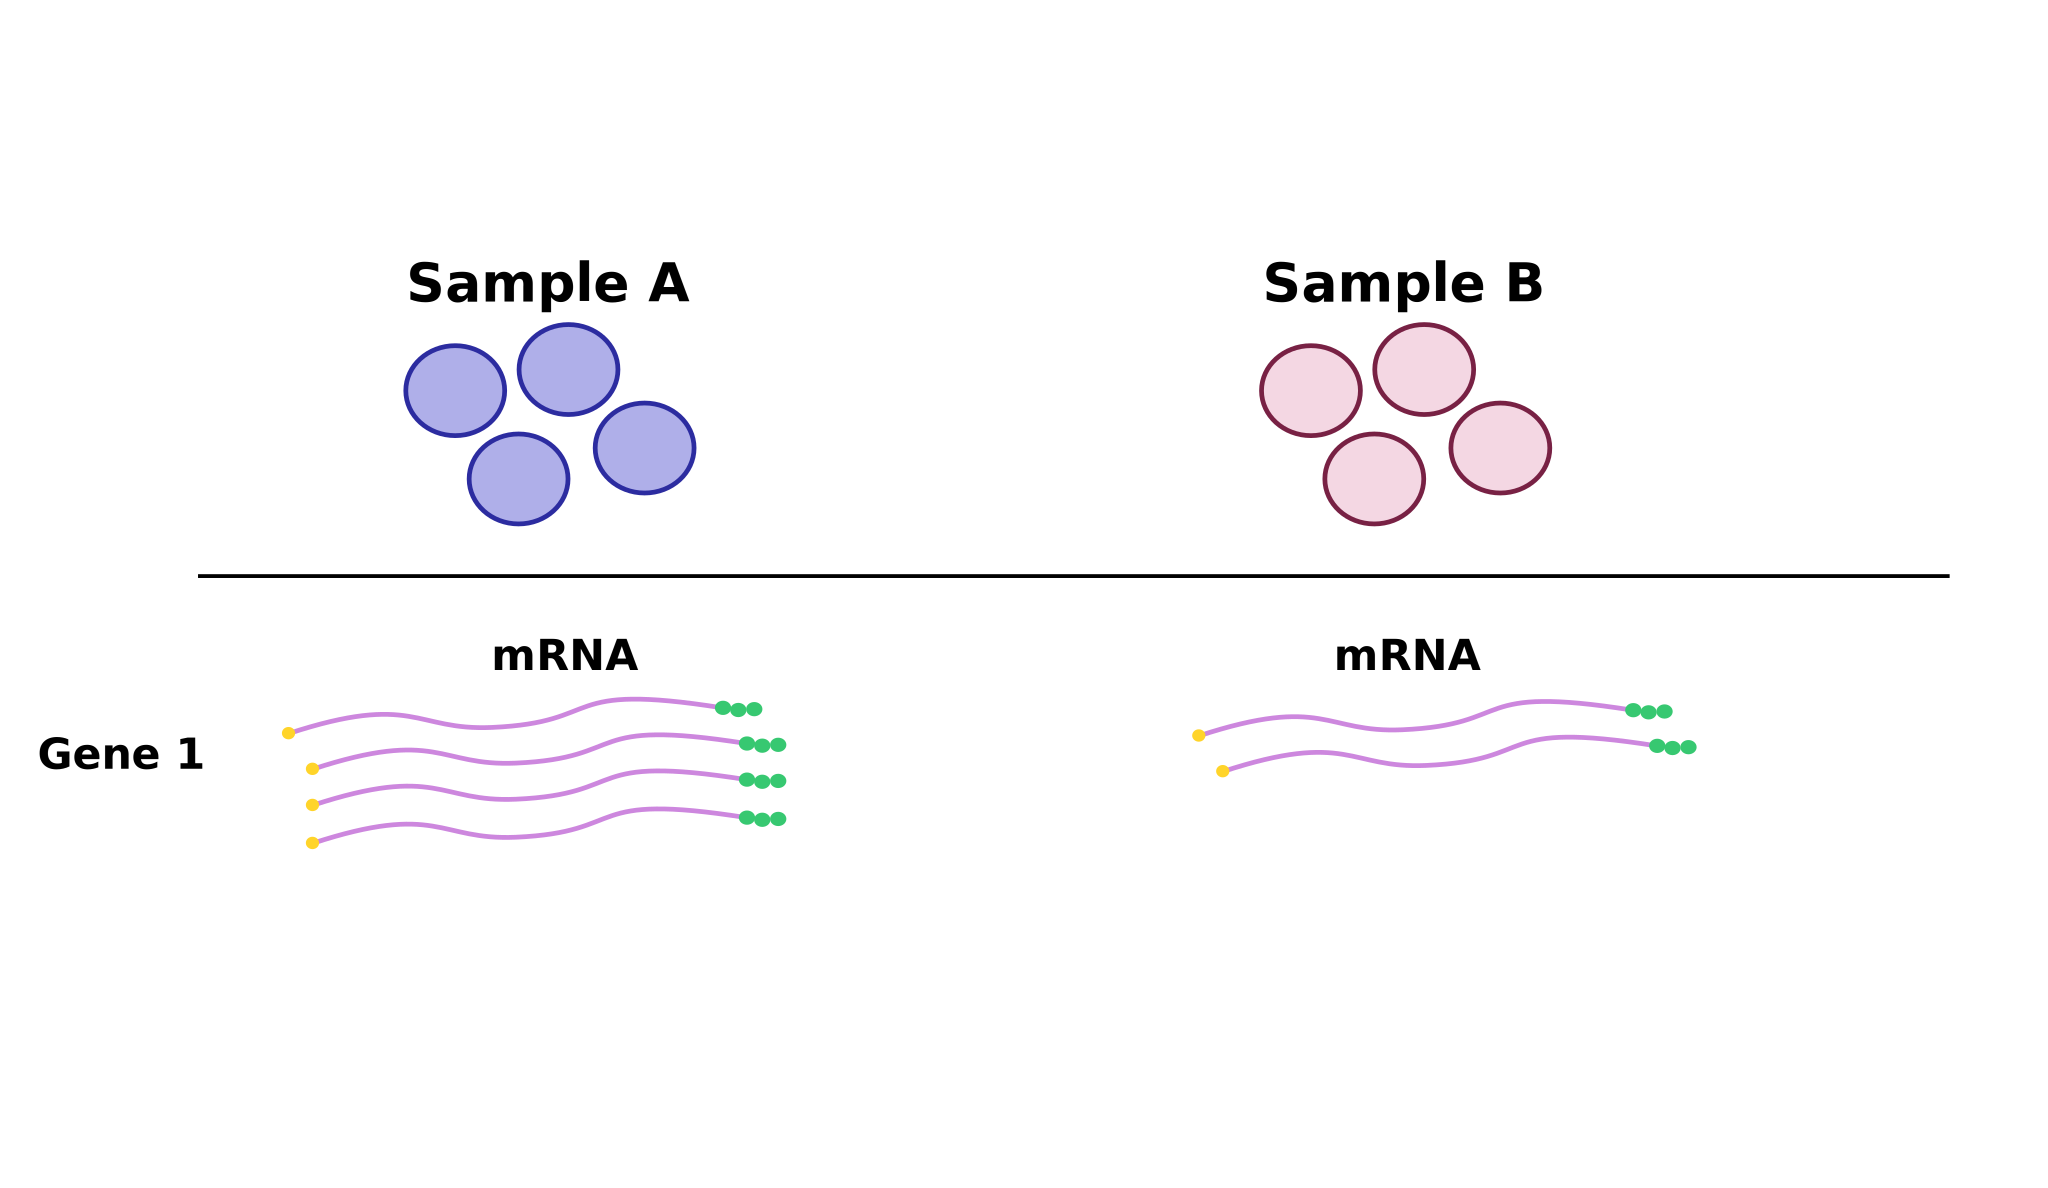
\includegraphics[width=\linewidth]{images/DE_0.pdf}
\vspace{-5em}
{\bf We cast the problem as a hypothesis test}
\begin{equation*}
H0 \quad : \quad \mu_A = \mu_B
\end{equation*}
\end{frame}

\begin{frame}
\frametitle{Static sampling methods are problematic for time-course analyses}
\begin{itemize}[label={$\bullet$}]
\item Large number of methods developped for identifying genes differentially
expressed between one or more static biological conditions.
\item These could be applied to time-course data, considering each time point
as a treatment.
\end{itemize}

\vspace{1em}
{\bf Why are those methods problematic for time-course analyses?}
\begin{itemize}[label={$\bullet$}]
\item Each treatment needs to be balanced.
\item Each treatment needs more than one replicate.
\item The time structure would essentially be ignored.
\end{itemize}

\vspace{1em}
{\bf Idea} \quad
Leverage functional analysis tools to represent the data as a function.
\end{frame}


\subsection{Differential analysis of timecourse data}

\begin{frame}
\frametitle{Representing the data as a function ``split-splines''}
\begin{figure}
\includegraphics[width=0.9\linewidth]{images/modeling_splitsplines.pdf}
\end{figure}
\end{frame}

\begin{frame}
\frametitle{Differential expression of time course data}

\vspace{2em}
{\bf Null hypothesis}: the two conditions can be represented by the same
function $f_0$
\\
{\bf Alternative hypothesis}: the data is better represented by two different
functions $f_1$.

\vspace{2em}
{\bf Log-likelihood ratio test}
\begin{equation}
F = \frac{SS^0 - SS^1}{SS^1}\,,
\end{equation}
with $SS^0 = \sum_i (y_i - f_0(y_i))^2$  and $SS^1 = \sum_i (y_i - f_1(y_i))^2$.
\end{frame}

\begin{frame}
\frametitle{Applying the differential analysis method on our data}

We test the following contrasts:
\begin{itemize}[label=${\bullet}$]
\item between drought and control, for the two genotypes: $C_{\text{drought}}^{\text{RTx430}} =
C_{\text{control}}^{\text{RTx430}}\,,$ and
$C_{\text{drought}}^{\text{BTx642}} = C_{\text{control}}^{\text{BTx642}}$

\item between the two genotypes in control:
$C_{\text{control}}^{\text{RTx430}} =
C_{\text{control}}^{\text{BTx642}}\,.$
\item between the two genotypes with respect to drought:
$C_{\text{control}}^{\text{RTx430}} - C_{\text{drought}}^{\text{RTx430}} = 
C_{\text{control}}^{\text{BTx642}} - C_{\text{drought}}^{\text{BTx642}}\,.$
\end{itemize}

\end{frame}

\begin{frame}
\frametitle{Results of global differential analysis}
{\bf 44\% of expressed genes
(10,727 genes) are detected as having a statistically significant change of at
least two log-fold change in at least one type of drought, sample type, or genotype  when
comparing drought versus control}

\vspace{2em}
{\scriptsize
\begin{tabular}{lllll}
\toprule
{} & \multicolumn{2}{c}{Root} & \multicolumn{2}{c}{Leaf} \\
{} & Preflowering & Postflowering & Preflowering & Postflowering \\
\midrule
Control-Drought RTx430    &          5977 &           4913 &          1889 &           2682 \\
Control-Drought BTx642    &          5457 &           3247 &          3231 &           1393 \\
Genotype specific drought &          1180 &            466 &           340 &            713 \\
\bottomrule
\end{tabular}

}
\end{frame}

\begin{frame}
\frametitle{Global responses to drought: leaves versus roots}
\begin{columns}
\begin{column}{0.6\linewidth}
\begin{itemize}[label={$\bullet$}]
\item Root reacts more strongly to drought, both in terms of shear numbers (~45\% of
genes expressed are found DE), and strength of response.
\item Difference seen immediately (21.7\% of the genes in root show immediate
response, while only 11\% in leaf).
\item Tolerant genotype have fewer genes DE in whatever drought they are tolerant
to.
\end{itemize}
\end{column}
\begin{column}{0.4\linewidth}
\begin{figure}
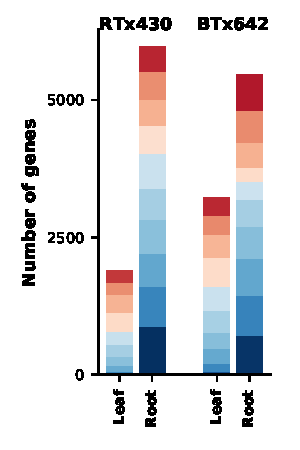
\includegraphics[width=0.8\linewidth]{figures/figure_2/fig2A_roots_versus_leaf.pdf}
\begin{center}
\caption{\small \textbf{Pre-flowering drought}}
\end{center}
\end{figure}
\end{column}
\end{columns}
\end{frame}

\begin{frame}
\frametitle{Global responses to drought: RTx430 versus BTx642}
\begin{itemize}[label={$\bullet$}]
\item 2,856 genes (11.56\% of expressed genes) with significantly different
transcriptional reactions to drought between the two genotypes.
\item Similar direction of response, but not same strength.
\item 518 genes that are virtually non-expressed in one of the genotypes.
\end{itemize}
\begin{center}
\begin{figure}
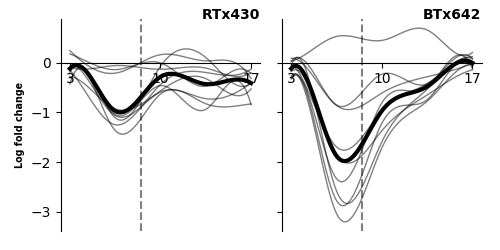
\includegraphics[width=0.6\linewidth]{figures/figure_2/geno_phenalynine.png}
\end{figure}
\end{center}
\end{frame}


\section{Clustering}

\begin{frame}
\frametitle{Clustering of time-course data}

{\color{Blue} \bf Motivation}
\begin{itemize}[label={$\bullet$}]
\item Any enrichment analysis (GO, pathway) we performed on the set of DE
genes showed very unstable enrichment;
\item Looking at the genes DE, many genes
displayed {\bf identical patterns}, but not on the same scale (and shift)
\end{itemize}

\vspace{2em}

{\color{Blue} \bf Idea}\quad Cluster the genes that behave the same way across
conditions and genotypes, to facilitate interpretation.

\end{frame}

\begin{frame}
\frametitle{Clustering of time course data}
\begin{figure}
\includegraphics[width=0.9\linewidth]{codes/images/gene_data.pdf}
\end{figure}
\end{frame}

\begin{frame}
\frametitle{Clustering of the time-course data}

\begin{itemize}[label={$\bullet$}]
\item Fit the ``split-splines'' regression for each gene;
\item Rescale the fitted values for each gene so that the expression is between 0 and 1;
\item Run k-means with a fixed number of clusters;
\item Estimate the ``goodness-of-fit'' for each gene $g$ and each cluster $k$:
{\footnotesize
\begin{equation}
S(g, k) =  \frac{1}{S_0(k)} \left(\underset{a_j, b_j}{\min}\sum_{j}
{\left(a_j y_i(t_j)
+ b_j - \mu^{C_j}_k(t_j)\right)}^2 \right)\,,
\end{equation}}
\item Assigned the top 50\% best genes to their closest centroid;
\end{itemize}

{\bf We apply this clustering strategy jointly across the genotypes, but for
each sample type \& drought type separately.}
\end{frame}

\begin{frame}
\frametitle{A wide variety of centroids}
\begin{columns}
\begin{column}{0.3\linewidth}
\center
\small
{\bf Leaf - Preflowering}
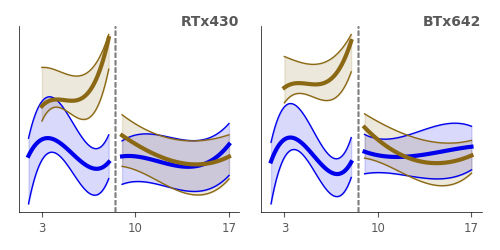
\includegraphics[width=0.9\linewidth]{figures/clusters/leaf_Preflowering_12.png}

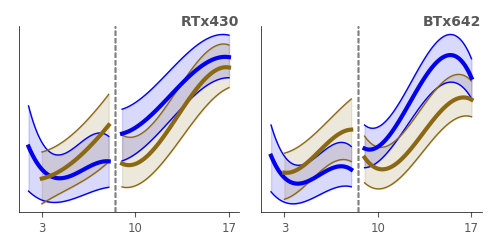
\includegraphics[width=0.9\linewidth]{figures/clusters/leaf_Preflowering_17.png}

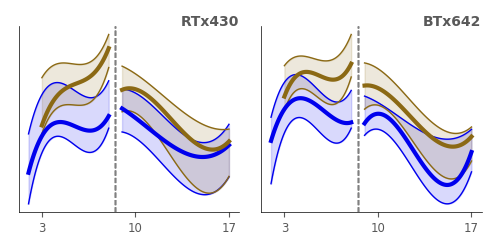
\includegraphics[width=0.9\linewidth]{figures/clusters/leaf_Preflowering_19.png}

\end{column}
\begin{column}{0.3\linewidth}
\center
\small
{\bf Root - Preflowering}
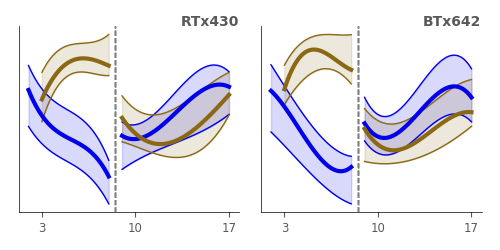
\includegraphics[width=0.9\linewidth]{figures/clusters/root_Preflowering_0.png}

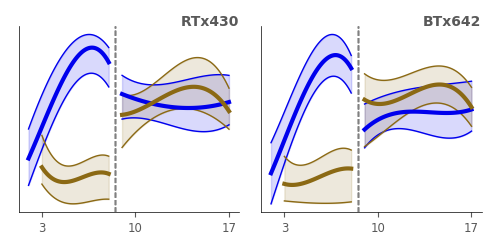
\includegraphics[width=0.9\linewidth]{figures/clusters/root_Preflowering_1.png}

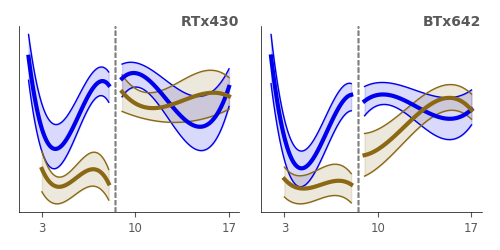
\includegraphics[width=0.9\linewidth]{figures/clusters/root_Preflowering_18.png}

\end{column}
\begin{column}{0.3\linewidth}
\center
\small
{\bf Root - Postflowering}
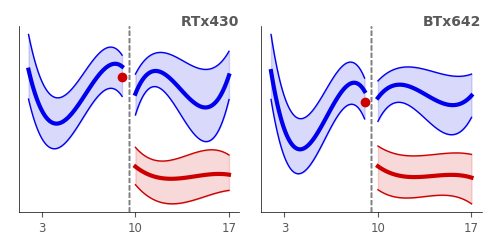
\includegraphics[width=0.9\linewidth]{figures/clusters/root_Postflowering_1.png}

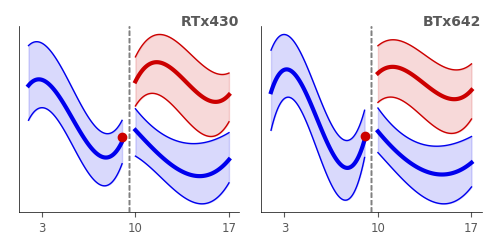
\includegraphics[width=0.9\linewidth]{figures/clusters/root_Postflowering_0.png}

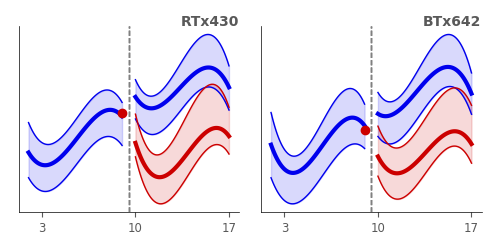
\includegraphics[width=0.9\linewidth]{figures/clusters/root_Postflowering_8.png}

\end{column}
\end{columns}
\end{frame}

\begin{frame}
\frametitle{Observations}
\begin{itemize}[label=$\bullet$]
\item Important differences between timepoints in drought and control;
\item In pre-flowering
\begin{itemize}[label=$\bullet$]
\item  many clusters resume to their ``control'' level, very
quickly after water resumes, but many clusters show recovery variations
\item Some clusters seem to have a shift. These may be {\bf developmental genes
cluster}.
\end{itemize}
\item Clusters are enriched in certain pathways \& GO terms
\end{itemize}
% XXX FIXME add more
\end{frame}

\begin{frame}
\frametitle{Many clusters show enrichment in stress responses}
\begin{columns}
\begin{column}{0.7\linewidth}
\begin{itemize}[label={$\bullet$}]
\item Response to ABA, response to oxidative stress, heat-shock proteins, programmed
cell-death related genes are up-regulated in stress.
\item Peroxidase family proteins (antioxidants produced in response to
oxidative stress) are down-regulated.
\item Genes homologous to the ABA receptor are downregulated (PYR6, HAB1, HAB2),
likely as a way to buffer ABA response.
\end{itemize}
\end{column}
\begin{column}{0.3\linewidth}
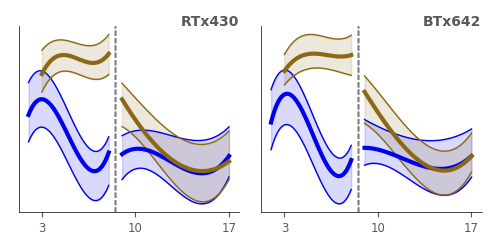
\includegraphics[width=\linewidth]{figures/clusters/root_Preflowering_14.png}

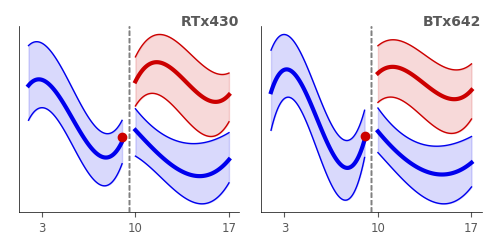
\includegraphics[width=\linewidth]{figures/clusters/root_Postflowering_0.png}
\end{column}
\end{columns}
\end{frame}


\begin{frame}
\frametitle{The Arbuscular mycorrhiza fungi symbiosis clusters}
\begin{columns}
\begin{column}{0.6\linewidth}
\begin{itemize}[label={$\bullet$}]
\item Two clusters are striking by the extent of the downregulation of the
genes.
\item They greatly overlap.
\item They contain most of the genes involved in the Arbuscular mycorrhiza fungi symbiosis 
\end{itemize}
\end{column}
\begin{column}{0.4\linewidth}
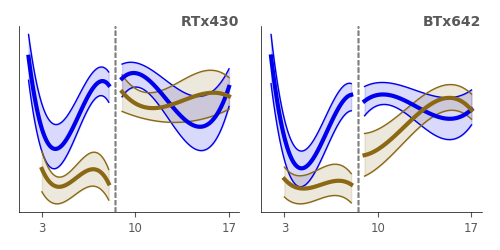
\includegraphics[width=0.9\linewidth]{figures/clusters/root_Preflowering_18.png}

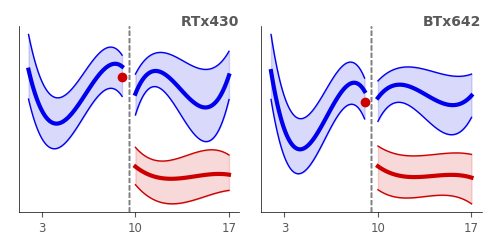
\includegraphics[width=0.9\linewidth]{figures/clusters/root_Postflowering_1.png}
\end{column}
\end{columns}
\end{frame}


\begin{frame}
\frametitle{The Arbuscular mycorrhiza fungi symbiosis}
\begin{columns}
\begin{column}{0.5\linewidth}
\begin{itemize}[label={$\bullet$}]
\item AM fungi penetrates the cortical cells of roots.
\item They help the plant
capture micronutrients such as phosphorus, nitrogren, sulphure.
\item In exchange, they receive carbon nutrient from the plant.
\end{itemize}
\end{column}
\begin{column}{0.5\linewidth}
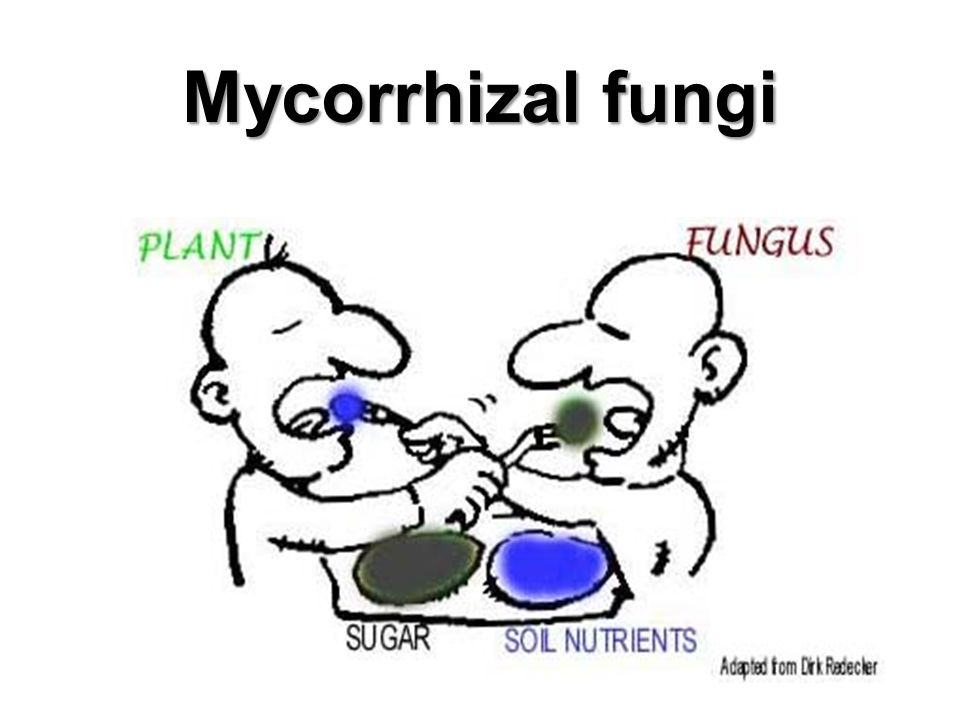
\includegraphics[width=\linewidth]{images/amf_symbiosis.jpg}
\end{column}
\end{columns}
\end{frame}

\begin{frame}
\frametitle{The AMF symbiosis under stress}
\begin{center}
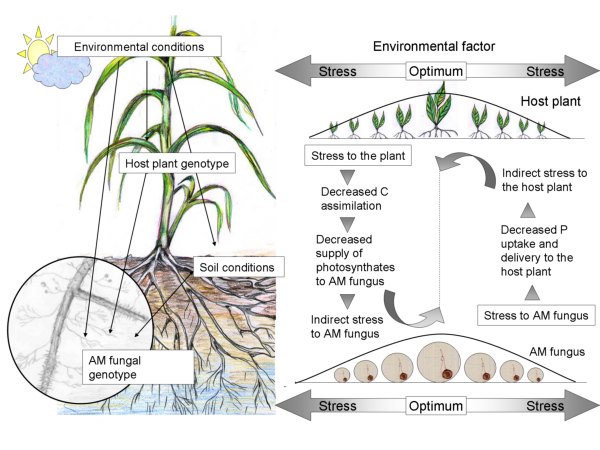
\includegraphics[width=0.8\linewidth]{images/amf_stress.png}
\end{center}
\end{frame}

\begin{frame}
\frametitle{The plant and AMF do not establish their symbiosis under drought
stress}
{\footnotesize
{\bf Hypothesis} The under-expression of those genes under drought suggests
that the plant and AMF do not establish this symbiotic relationship.}
\vspace{1em}

{\bf Validation}
\begin{itemize}[label={$\bullet$}]
\footnotesize
\item We measure total fungi abundance in the roots of our samples
under drought by performing PCR quantification with 18S amplification.
\item We measure relative AMF abundance to total fungi abundance using ITS
sequencing.
\item We then estimate total AMF abundance in the roots
\end{itemize}

\begin{center}
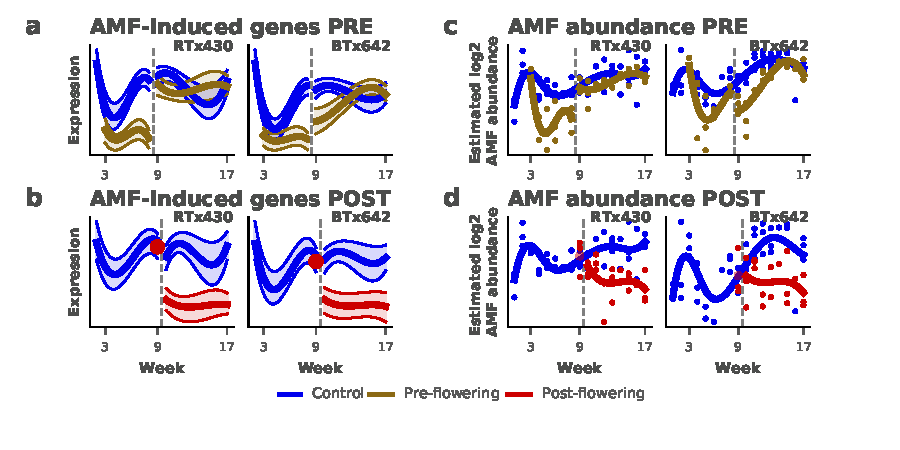
\includegraphics[width=0.6\linewidth]{figures/figure_5.pdf}
\end{center}
\end{frame}


\begin{frame}
\frametitle{Conclusion}
\textbf{\color{Blue} Conclusion}
\begin{itemize}[label={$\bullet$}]
\item First longitudinal study of drought stress on plants.
\item Largest cohesive transcriptomic data in plants.
\item \textit{S. bicolor} detects and adapts to drought stress extremely rapidly
\item Using a wide variety of molecular mechanisms
\item Better insights in molecular mecanisms behind the stay-green phenotype
\end{itemize}

\vspace{1em}
{\footnotesize
\textbf{\color{Blue} Related publications}
\begin{itemize}[label={$\bullet$}]
\item Varoquaux et al, (accepted), ``Transcriptomic analysis of field-droughted
sorghum from seedling to maturity reveals biotic and metabolic responses.''
\item Varoquaux \& Purdom (in prep), ``A pipeline to analyse time-course gene
expression data''
\end{itemize}}
\end{frame}


\begin{frame}
\frametitle{}
\vspace{4em}
{\bf \Large A statistical model for time-course transcriptomic data clustering}
\begin{flushright}
\footnotesize
\em Nelle Varoquaux, Stephanie De Graaf, Elizabeth Purdom
\end{flushright}
\end{frame}

\begin{frame}
\frametitle{A statistical model for clustering time-course transcriptomic data}
  

\textbf{\color{Blue} Goal} \quad Develop a robust clustering method for
time-course data to cluster genes co-regulated together.


\textbf{\color{Blue} Idea} \quad Model centroids by a function and leverage mixture
models.

\vspace{-2em}
\only<1>{%
\begin{figure}
\includegraphics[width=0.65\linewidth]{codes/images/splines_data.pdf}
\end{figure}}
\only<2>{%
\begin{figure}
\includegraphics[width=0.65\linewidth]{codes/images/splines_modeling.pdf}
\end{figure}}
\only<3>{%
\begin{figure}
\includegraphics[width=0.65\linewidth]{codes/images/gene_data.pdf}
\end{figure}}
\only<4->{%
\begin{figure}
\includegraphics[width=0.65\linewidth]{codes/images/scaled_centroids.pdf}
\end{figure}
}

\end{frame}
\begin{frame}
\frametitle{The ``splines'' mixture model}

\begin{figure}
\includegraphics[width=0.65\linewidth]{codes/images/scaled_centroids.pdf}
\end{figure}

\begin{overlayarea}{12cm}{5cm}
{\bf \small Clustering via a constrained mixture model}
\vskip-1.3ex
\rule{\dimexpr\paperwidth-1.5cm\relax}{0.4pt}
\begin{equation*}
\underbrace{y_{ij}}_{\text{\tiny data}} \quad \sim \quad \sum_k \quad
\underbrace{\pi_k}_{\text{\tiny mixture coefficient}}
\quad \mathcal{N}\large(a_{ik}\underbrace{\mu_k(t_j)}_{\text{\tiny
centroid, $\text{min}\mu(t_j) = 0$, $\text{max}\mu(t_j) = 1$}} +
b_{ik}, \sigma^2_{ikt}\large)
\end{equation*}

\end{overlayarea}
\end{frame}

\begin{frame}
\frametitle{Comparing methods}

\textbf{\color{Blue} Methods} \quad Kmeans, splines-KMeans, Splines-GMM,
Splines-NBMM, Splines-ZINBMM

\vspace{1em}
\textbf{\color{Blue} Simulated datasets} \quad 5 Datasets of 16 clusters,
including a cluster with no changes overtime.

\vspace{1em}
\textbf{\color{Blue} ``Real'' datasets} \quad
\begin{itemize}[label={$\bullet$}]
\item \citet{shoemaker:ultrasensitive} mouse lung tissue infected with 4
strains of influenza + a control condition, 14 timepoints
\item \citet{varoquaux:transcriptomic} leaf and root tissue, of two genotypes,
two drought condition + a well-watered, 15 timepoints.
\end{itemize}

\vspace{1em}
\end{frame}

\begin{frame}
\frametitle{Preliminary results on real data}
\textbf{\color{Blue} Validation method}
\begin{itemize}[label={$\bullet$}]
\item Consider each replicate as a different gene which we denote as
\textit{``pseudo-gene''};
\item Run the clustering;
\item Count the number of times two ``pseudo-genes'' are not in the same
cluster.
\end{itemize}
\begin{figure}
\includegraphics[width=0.6\linewidth]{figures/varoquaux2019_leaf_replicates.pdf}
\end{figure}
\end{frame}

\begin{frame}
\frametitle{Clustering of gene expression time-course data}
\begin{figure}
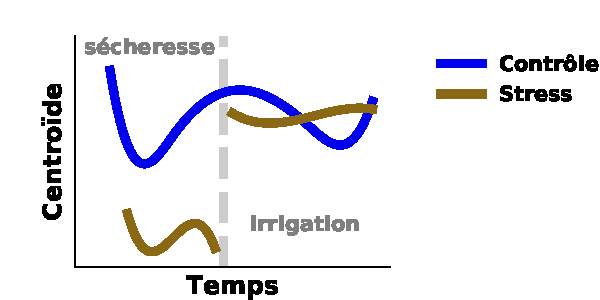
\includegraphics[width=0.6\linewidth]{figures/amf_centroids.pdf}
\end{figure}

\vspace{1.5em}
\begin{overlayarea}{12cm}{5cm}
\only<2->{%
{\bf \small Genes involved in arbuscular mycorrhizal symbiosis are
co-regulated}
\vskip-1.3ex
\rule{\dimexpr\paperwidth-1.5cm\relax}{0.4pt}
\begin{figure}
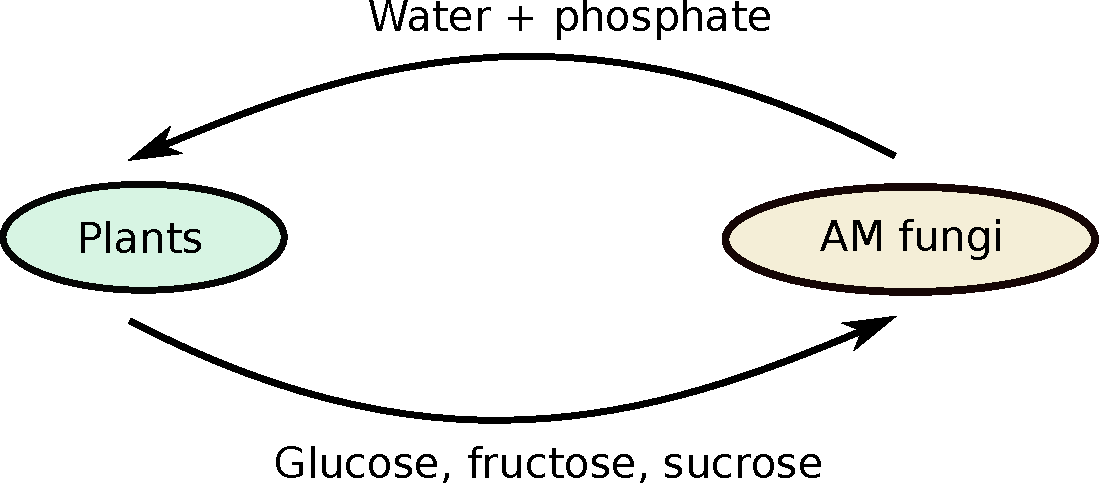
\includegraphics[width=0.5\linewidth]{schemas/symbiose_amf.pdf}
\end{figure}}
\end{overlayarea}
\end{frame}




\begin{frame}
\frametitle{Conclusion \& Future work}

\textbf{\color{Blue} Conclusion} Preliminary results show better performance
on simulated data \& increased \textbf{stability
on real data}.

\vspace{2em}
\textbf{\color{Blue} Future work}
\begin{itemize}[label={$\bullet$}]
\item More experiments on stability of the results (bootstrap) and inclusion
of a method to choose the number of cluster;
\item Detection of clusters ``highly'' differentially expressed.
\item Biological interpretation of the root EPICON dataset, with the hope of
finding anti-correlated genes belonging to specific pathways (biotic and
abiotic stress)
\end{itemize}

\end{frame}


\begin{frame}
\frametitle{Acknowledgments}
\begin{center}
\begin{columns}
\begin{column}{0.3\linewidth}
\scriptsize
{\bf Purdom lab} \\
Boying Gong \\
Stephanie DeGraaf \\
\vspace{1em}
{\bf Lemaux lab} \\
Mary Madera \\
Judith \\
Claudia\\
Grady Pierroz\\
\vspace{1em}
{\bf Niyogi lab} \\
Chris Baker \\
Dhruv Patel \\
Tim Jeffers 
\end{column}
\begin{column}{0.3\linewidth}
\scriptsize
{\bf JGI} \\
John Vogel \\
Ronan O'malley \\
Axel Visel \\
Ben Cole \\
Matthew Blow \\
\vspace{1em}
{\bf Microbiome \& fungi} \\
Devin Coleman-Derr\\
John Taylor \\
Cheng Gao
\end{column}

\begin{column}{0.3\linewidth}
\scriptsize
{\bf BIDS} \\
Alexandra Paxton \\
Diya Das \\
Ciera Martinez
\end{column}
\end{columns}
\end{center}

\begin{center}
\hspace*{-1.5em}
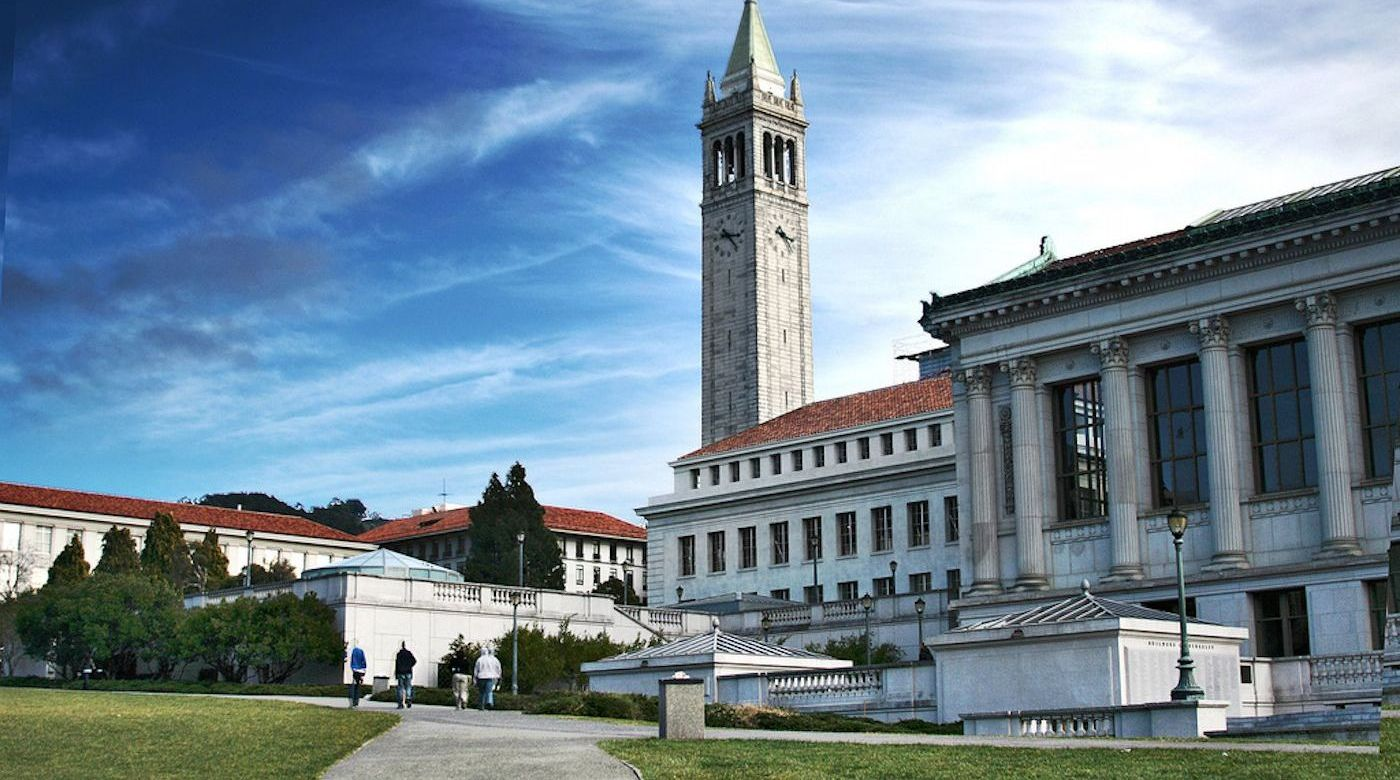
\includegraphics[width=1.1\linewidth]{images/berkeley_campanile.jpeg}
\end{center}
\end{frame}

\begin{frame}[allowframebreaks,noframenumbering]
    \frametitle{References}
    \bibliographystyle{plainnat}
    \bibliography{biblio}
\end{frame}

\end{document}

